\documentclass[11pt]{article}
\usepackage{algorithm}
\usepackage{algpseudocode}
\usepackage{algorithmicx}
\usepackage{amsmath}
\usepackage{graphicx}

\begin{document}
\title{Homework 1 of Numeric Linear Algebra}
\date{2017/9/24}
\author{Ziheng Chen, 1500010632}
\maketitle

1. (1.2) We give the following algorithm:
\begin{algorithm}[H]
\caption{Solve $(ST-\lambda I)x=b$}
\begin{algorithmic}[1]
\State $ x(n) = b(n) / (T(n, n) \cdot S(n, n) - \lambda) $
\State $ Tc(n) = T(n, n) \cdot x(n) $
\For{$ k=n-1:1 $}
	\State $ tmp = T(k,k+1:n) \cdot x(k+1,n) $
	\State $ x(k) = (b(k)-S(k,k+1:n)\cdot Tc(k+1:n)-S(k,k)\cdot tmp) / (S(k,k)\cdot T(k,k)-\lambda) $
	\State $ Tc(k) = tmp + T(k,k) \cdot x(k) $
\EndFor
\end{algorithmic}
\end{algorithm}
Total time complexity of the algorithm is $2 n^2 + 4n - 2$.
\\\\
2. (1.4) For the vector changes from the second row, we take Gauss vector $l_1 = (0, -2, -2)^T$ and the Gauss transform is calculated as follows:
$$ L_k = I - l_k e_k^T = \begin{bmatrix} 1 & 0 & 0 \\ 2 & 1 & 0 \\ 2 & 0 & 1 \\ \end{bmatrix}. $$
\\\\
3. (1.6) Notice that 
$$ \begin{bmatrix}1 & 0 & \cdots & 0 & 1 \\ -1 & 1 & \cdots & 0 & 1 \\ \vdots & \vdots & \ddots & \vdots & \vdots \\ -1 & -1 & \cdots & 1 & 1 \\ -1 & -1 & \cdots & -1 & 1\end{bmatrix}
= L U
= \begin{bmatrix}1 & 0 & \cdots & 0 & 0 \\ -1 & 1 & \cdots & 0 & 0 \\ \vdots & \vdots & \ddots & \vdots & \vdots \\ -1 & -1 & \cdots & 1 & 0 \\ -1 & -1 & \cdots & -1 & 1\end{bmatrix}
\times \begin{bmatrix}1 & 0 & \cdots & 0 & 1 \\ 0 & 1 & \cdots & 0 & 2 \\ \vdots & \vdots & \ddots & \vdots & \vdots \\ 0 & 0 & \cdots & 1 & 2^{n-2} \\ 0 & 0 & \cdots & 0 & 2^{n-1}\end{bmatrix}.$$
\\\\
4. (1.8) Consider the $(k-1)$-th row of $A_2$ : $(0, b_2, \cdots, b_n)$, where $b_i=a_{ki}-a_{k1}\cdot \frac{a_{1i}}{a_{11}}$, is restricted by the two following inequalities:
$$ |a_{11}| > \sum_{i=2}^{n} |a_{1i}| $$
$$ |a_{kk}| > \sum_{i=1, i\neq k}^{n} |a_{ki}|,$$
so we have
\begin{align*}
|b_k| = |a_{kk} - a_{k1} \cdot \frac{a_{1k}}{a_{11}}|
& \ge |a_{kk}| - |a_{k1}| \cdot \frac{|a_{1k}|}{|a_{11}|} \\
& > \left( \sum_{i=1, i\neq k}^{n} |a_{ki}| \right) + \frac{|a_{k1}|}{|a_{11}|} \cdot \left( -|a_{11}| + \sum_{i=2, i\neq k}^{n} |a_{1i}| \right) \\
& = \sum_{i=2, i\neq k}^{n} \left( |a_{ki}| + \frac{|a_{k1}|}{|a_{11}|} \cdot |a_{1i}| \right) \\
& \ge \sum_{i=2, i\neq k}^{n} |b_i|.
\end{align*}
Therefore $A_2$ is still diagonally dominant.
\\\\
5. (1.11) Suppose $A_{11}$ has decomposition $A_{11} = LU$. Then after the $k$-th Gaussian elimination, we should have
$$\begin{bmatrix}L^{-1} & 0 \\ L_k & I_{n-k} \end{bmatrix} \begin{bmatrix}A_{11} & A_{12} \\ A_{21} & A_{22} \end{bmatrix} = \begin{bmatrix}U & * \\ 0 & U_k \end{bmatrix}$$
where $L_k$ is subject to $L_k \cdot A_{11} + A_{21} = 0$.
Since $A_{11}$ is invertible, so $L_k = A_{21} \cdot A_{11}^{-1}$ and $U_k = -A_{21}\cdot A_{11}^{-1}\cdot A_{12} + A_{22} = S$.
\\\\
\newpage
6. (1c.1) We have the following numerical result; see table \ref{tab:t_6}.
\begin{table}[ht]
	\caption{Gaussian Method Error}
	\label{tab:t_6}
	\centering
	\begin{tabular}{c|cc}
		\hline
		& $||x^*-x||$ & $||Ax^*-b||$ \\
		\hline
		normal   & 7.259e+08 & 1.666e-08 \\
		improved & 8.597e-08 & 1.776e-15 \\
		\hline
	\end{tabular}

	\emph{Note: $Cond(A)=8.427694\times 10^{16}$}
\end{table}

With the visual comparison of error in each component between two methods, we can have a rough idea of the accuracy of the improved method; see figure \ref{fig:f_6}
\begin{figure}[ht]
	\centering
	\label{fig:f_6}
	\caption{Problem 6}
	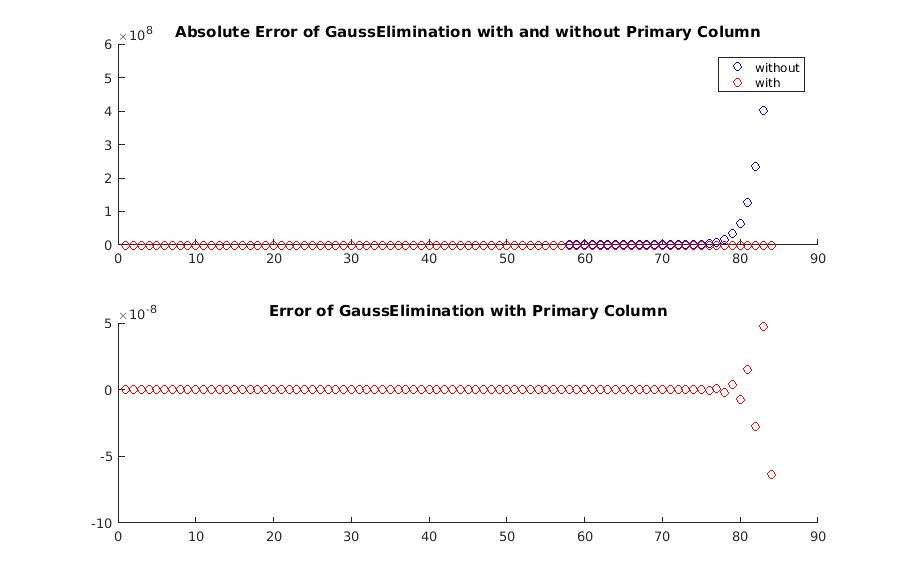
\includegraphics[width=\textwidth]{gaussian.jpg}
\end{figure}

In sum, the normal Gaussian Elimination has a rather low numerical precision, compared with the improved method of choosing the largest column element.
\\\\
\newpage
7. (1c.2) For the first part of the question, we set $b$ as a random vector with each component conforming the uniform distribution $U(0, 1)$.
Since the problem is well-conditioned ($cond(A)=1.499698$) , we can trust that $x = A \backslash b$ gives out a true solution.
The result is followed in the description below.
\begin{table}[ht]
	\caption{Cholesky Method Error(Part 1)}
	\centering
	\begin{tabular}{c|cc}
		\hline
		& $||x^*-x||$ & $||Ax^*-b||$ \\
		\hline
		normal   & 3.298e-17 & 8.467e-16 \\
		improved & 8.375e-17 & 5.033e-16 \\
		\hline
	\end{tabular}
	
	\emph{Note: $Cond(A)=1.499698\times 10^{0}$}
\end{table}

\begin{figure}[ht]
	\centering
	\caption{Problem 7.1}
	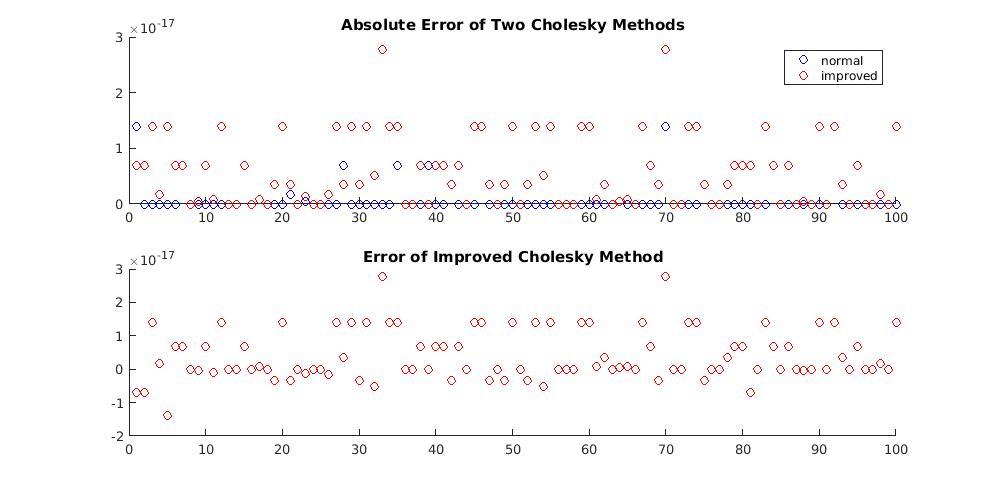
\includegraphics[width=\textwidth]{cholesky1.jpg}
\end{figure}

Although the improved method has a less accurate solution (in terms of distance to the true solution), it is a better approximation if compared in terms of $||Ax^*-b||$ distance.
But, in the sense of precision, both methods are quite accurate due to the well-condition of the problem.
\\\\
\newpage
As for the second part, we can easy solve the equation and get the solution : $x = (1, 1 \dots , 1)^T$. 
Then, we compare both methods and examine the result.
\begin{table}[ht]
	\caption{Cholesky Method Error(Part 2)}
	\centering
	\begin{tabular}{c|cc}
		\hline
		& $||x^*-x||$ & $||Ax^*-b||$ \\
		\hline
		normal   & 7.457e+07 & 2.231e-04 \\
		improved & 1.677e+02 & 3.447e-15 \\
		\hline
	\end{tabular}
	
	\emph{Note: $Cond(A)=6.155604\times 10^{18}$}
\end{table}

\begin{figure}[ht]
	\centering
	\caption{Problem 7.2}
	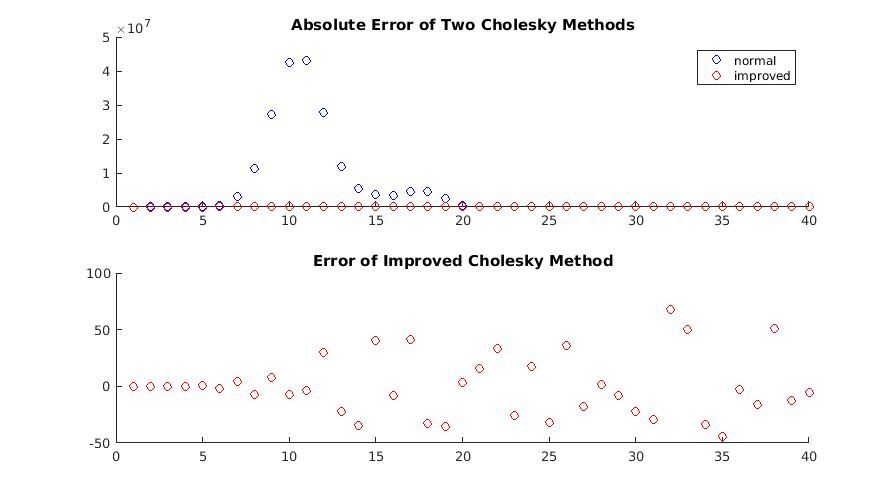
\includegraphics[width=\textwidth]{cholesky2.jpg}
\end{figure}

As is shown in the table, neither of the two can solve out an accurate solution(because of the illness in the problem); but, in the sense of mapped error $||Ax^*-b||$, the improved method performs quite satisfying.
\end{document}